%%%%%%%%%%%%%%%%%%%%%%%%%%%%%%%%%%%%%%%%%%%%%%%%%%%%%%%%%%%%%%%%%%%%%%%%%%%%%%%%
%2345678901234567890123456789012345678901234567890123456789012345678901234567890
%        1         2         3         4         5         6         7         8

\documentclass[letterpaper, 10 pt, conference]{ieeeconf}  % Comment this line out if you need a4paper

%\documentclass[a4paper, 10pt, conference]{ieeeconf}      % Use this line for a4 paper

\IEEEoverridecommandlockouts                              % This command is only needed if
                                                          % you want to use the \thanks command

\overrideIEEEmargins                                      % Needed to meet printer requirements.

\usepackage{graphicx}
\usepackage{amsmath}
\usepackage{amssymb}
\usepackage{booktabs}
\usepackage{multirow}
\usepackage{xcolor}
\usepackage{cite}
\usepackage{eso-pic}
\usepackage{tikz}
\usetikzlibrary{positioning,arrows.meta,fit,backgrounds,calc,shapes.geometric}
\definecolor{cBlue}{HTML}{2A78D6}
\definecolor{cOrange}{HTML}{EB6834}
\definecolor{cAqua}{HTML}{1BAF7A}
\definecolor{cViolet}{HTML}{4A3AA7}
\definecolor{cRed}{HTML}{E34948}
\definecolor{cGray}{HTML}{9A9893}
\definecolor{cDark}{HTML}{0B0B0B}
\definecolor{cMuted}{HTML}{52514E}
\definecolor{cGrid}{HTML}{E4E3DF}

\usepackage[hidelinks]{hyperref}

\graphicspath{{figures/}}
\newcommand{\todo}[1]{{\color{cRed}[#1]}}

% draft banner on every page
\AddToShipoutPictureBG{%
  \AtPageUpperLeft{\raisebox{-0.9cm}{\makebox[\paperwidth]{\footnotesize\sffamily\color{cRed}%
  DRAFT \,--\, prepared for publication, not yet peer reviewed \,--\, \today}}}}

\title{\LARGE \bf
Autonomous Suturing Task:\\
From Hierarchical Policies in Simulation to a Guarded\\
Needle-Handling Pipeline on a Real dVRK
}

\author{Xiangrui Sun$^{1}$, Jiaming Wen$^{2}$, Adnan Munawar$^{1,\dagger}$, and Anqi Liu$^{3,\dagger}$% <-this % stops a space
\thanks{*This work was not supported by any organization}% <-this % stops a space
\thanks{\textbf{Draft manuscript prepared for publication.} Results, figures and text are
        preliminary and subject to change.}%
\thanks{$^{\dagger}$Corresponding authors: Adnan Munawar {\tt\small amunawa2@jhu.edu};
        Anqi Liu {\tt\small aliu.cs@jhu.edu}.}%
\thanks{$^{1}$Xiangrui Sun and Adnan Munawar are with the Laboratory for Computational
        Sensing and Robotics, Johns Hopkins University, Baltimore, MD 21218, USA
        {\tt\small xsun97@jh.edu}}%
\thanks{$^{2}$Jiaming Wen is with \todo{affiliation}
        {\tt\small \todo{email}}}%
\thanks{$^{3}$Anqi Liu is with the Department of Computer Science,
        Johns Hopkins University, Baltimore, MD 21218, USA}%
}


\begin{document}



\maketitle
\thispagestyle{empty}
\pagestyle{empty}


%%%%%%%%%%%%%%%%%%%%%%%%%%%%%%%%%%%%%%%%%%%%%%%%%%%%%%%%%%%%%%%%%%%%%%%%%%%%%%%%
\begin{abstract}
Reinforcement-learning (RL) policies for surgical suturing are commonly trained
and scored in simulation and seldom run on a physical robot. We report our
progress in moving the hierarchical suturing policies of SurgicAI onto a da Vinci
Research Kit (dVRK). First, we re-run the original five-stage hierarchy
(Approach, Place, Insert, Regrasp, Pullout) on ROS~2 and AMBF~3 without changing
any policy or environment logic. It completes the full suture in 11 of 20
episodes, against the 52\% reported by its authors. Second, we build a perception
front end for the real endoscope. Depth Anything V2 is fine-tuned on simulated
RGB--depth pairs so that it outputs metric depth, and FoundationPose uses that
depth to estimate the pose of the needle. An ArUco-based hand-eye calibration
improves PSM localization from about 5\,cm to 5--10\,mm. Third, we deploy the
released policies on a real PSM through an explicit observation--action
contract. Running the policies against their own demonstrations exposed three
silent mismatches between the training environment and a straightforward
deployment: the Euler-angle branch, the action scale, and whether the
observation is open- or closed-loop. Once these are fixed, the released Approach
checkpoint reproduces 45 of its 50 demonstrations. We also show that the gap
between the training workspace and the real task can be closed by staging the
start pose rather than by retraining, and we describe a guarded phase machine
that takes the arm from staging through grasp, lift and transport to the suture
entry pose. Finally, we propose a two-stage grasp calibration, in which a
Bernstein residual field corrects a coarse FoundationPose-based grasp target,
and report the first ten hardware samples. They reveal a constant offset of
about 43\,mm that must be removed before any fit.
\end{abstract}


%%%%%%%%%%%%%%%%%%%%%%%%%%%%%%%%%%%%%%%%%%%%%%%%%%%%%%%%%%%%%%%%%%%%%%%%%%%%%%%%
\section{INTRODUCTION}

Suturing is the canonical benchmark for surgical autonomy. It is long-horizon,
contact-rich, and needs millimetre precision on a thin, curved,
near-symmetric object. Simulation platforms built on AMBF~\cite{munawar2019ambf}
and the Surgical Robotics Challenge (SRC)~\cite{munawar2022src} have made the
task learnable. SurgicAI~\cite{wu2024surgicai} splits it into five subtasks and
learns a policy for each one. A high-level policy then sequences them, and the
full chain succeeds far more often with this hierarchy than with a flat policy.
Physical deployments remain rare. Orbit-Surgical transferred a policy to a real
dVRK at 50\% on needle lift~\cite{yu2024orbit}, and a recent review describes the
field as ``mature at the simulation stage but \ldots\ preclinical''~\cite{review2026rl}.

This draft reports what it has taken so far to move the SurgicAI policies onto a
real dVRK~\cite{kazanzides2014dvrk} Patient Side Manipulator (PSM). We emphasize
where the transfer actually broke. Much of the gap turned out not to be
``sim-to-real'' in the usual sense. The cause was usually an unstated convention
in the training code that a deployment has to reproduce exactly. Our
contributions are:
\begin{enumerate}
\item A \emph{replication} of the hierarchical suturing pipeline on ROS~2/AMBF~3.
      The environment and policy code are unchanged, and the chained success rates
      are consistent with the published ones (Sec.~\ref{sec:hier}).
\item A \emph{perception front end} for the real endoscope: sim-supervised metric
      depth, FoundationPose needle tracking and hand-eye registration of the PSM
      (Sec.~\ref{sec:perception}).
\item A \emph{verified deployment contract} for the released checkpoints. It
      identifies three defects that invalidate a straightforward deployment, and
      a staging solve that places any real grasp inside the trained support
      (Sec.~\ref{sec:deploy}).
\item A \emph{guarded real-robot phase machine} and the hardware findings from
      bringing it up, including the PSM position deadband
      (Sec.~\ref{sec:sequence}).
\item A \emph{two-stage grasp calibration} whose structure is predicted from the
      dVRK kinematics before any data is collected, together with the first
      hardware samples (Sec.~\ref{sec:calib}).
\end{enumerate}
Fig.~\ref{fig:overview} shows how the components fit together.

\begin{figure*}[t]
  \centering
  \resizebox{\textwidth}{!}{% System overview. Included with \input; needs tikz libraries
% positioning, arrows.meta, fit, backgrounds, calc.
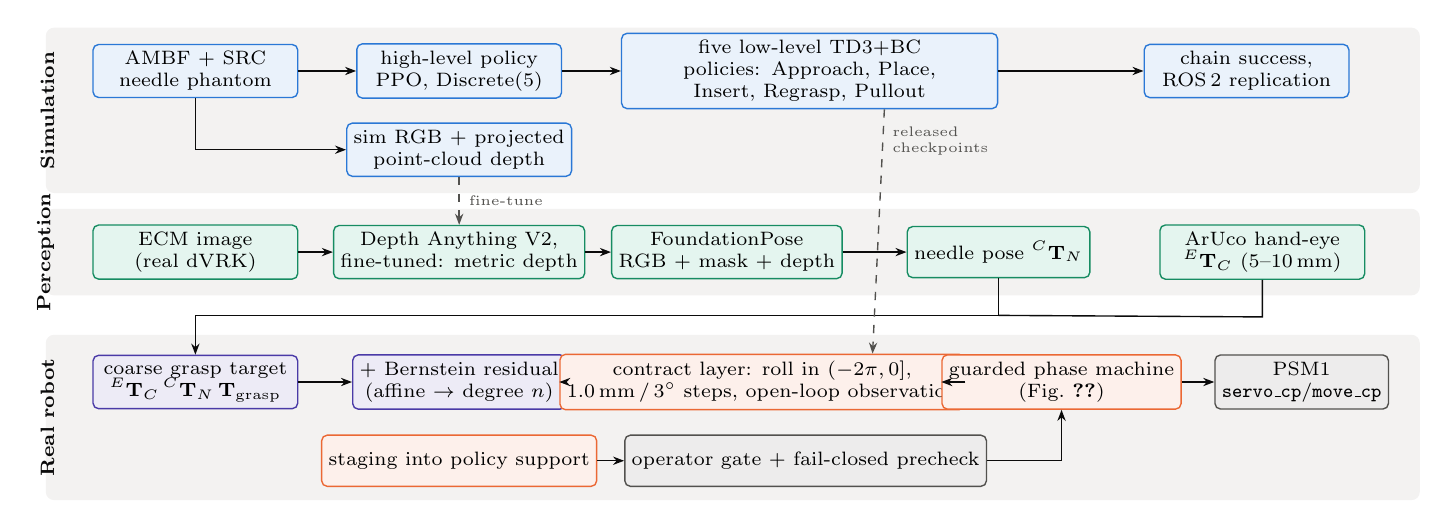
\begin{tikzpicture}[
  font=\scriptsize,
  >={Stealth[length=4pt]},
  box/.style={draw=cMuted, rounded corners=2pt, fill=white, align=center,
              inner sep=2.5pt, minimum height=6.5mm, line width=0.5pt},
  sim/.style={box, fill=cBlue!10, draw=cBlue},
  per/.style={box, fill=cAqua!12, draw=cAqua!80!black},
  cal/.style={box, fill=cViolet!10, draw=cViolet},
  dep/.style={box, fill=cOrange!10, draw=cOrange},
  hw/.style={box, fill=cGray!18, draw=cMuted},
  flow/.style={->, draw=cDark, line width=0.5pt},
  dashflow/.style={->, draw=cMuted, dashed, line width=0.5pt},
  tag/.style={font=\tiny, text=cMuted, align=center},
  lanetitle/.style={font=\scriptsize\bfseries, text=cDark, rotate=90, anchor=south},
]
% ---- lanes (drawn first)
\fill[cGrid!45, rounded corners=3pt] (-0.35, 0.55) rectangle (17.1, -1.55);
\fill[cGrid!45, rounded corners=3pt] (-0.35,-1.75) rectangle (17.1, -2.85);
\fill[cGrid!45, rounded corners=3pt] (-0.35,-3.35) rectangle (17.1, -5.45);
\node[lanetitle] at (-0.12,-0.5) {Simulation};
\node[lanetitle] at (-0.12,-2.3) {Perception};
\node[lanetitle] at (-0.12,-4.4) {Real robot};

% ---- simulation
\node[sim, minimum width=26mm] (ambf) at (1.55,0) {AMBF + SRC\\needle phantom};
\node[sim, minimum width=26mm] (hlp) at (4.9,0) {high-level policy\\PPO, Discrete(5)};
\node[sim, text width=46mm] (llp) at (9.35,0)
  {five low-level TD3+BC policies: Approach, Place,\\Insert, Regrasp, Pullout};
\node[sim, minimum width=26mm] (bench) at (14.9,0) {chain success,\\ROS\,2 replication};
\node[sim, minimum width=26mm] (dadata) at (4.9,-1.0) {sim RGB + projected\\point-cloud depth};
\draw[flow] (ambf) -- (hlp);
\draw[flow] (hlp) -- (llp);
\draw[flow] (llp) -- (bench);
\draw[flow] (ambf.south) |- (dadata.west);

% ---- perception
\node[per, minimum width=26mm] (ecm) at (1.55,-2.3) {ECM image\\(real dVRK)};
\node[per, minimum width=26mm] (da) at (4.9,-2.3) {Depth Anything V2,\\fine-tuned: metric depth};
\node[per, minimum width=26mm] (fp) at (8.3,-2.3) {FoundationPose\\RGB + mask + depth};
\node[per, minimum width=22mm] (needle) at (11.75,-2.3) {needle pose ${}^{C}\mathbf{T}_{N}$};
\node[per, minimum width=26mm] (aruco) at (15.1,-2.3) {ArUco hand-eye\\${}^{E}\mathbf{T}_{C}$ (5--10\,mm)};
\draw[flow] (ecm) -- (da);
\draw[flow] (da) -- (fp);
\draw[flow] (fp) -- (needle);
\draw[dashflow] (dadata) -- node[right, tag]{fine-tune} (da);

% ---- real robot: calibration + deployment
\node[cal, minimum width=26mm] (coarse) at (1.55,-3.95) {coarse grasp target\\${}^{E}\mathbf{T}_{C}\,{}^{C}\mathbf{T}_{N}\,\mathbf{T}_{\mathrm{grasp}}$};
\node[cal, minimum width=26mm] (fine) at (4.9,-3.95) {+ Bernstein residual\\(affine $\rightarrow$ degree $n$)};
\node[dep] (contract) at (8.75,-3.95)
  {contract layer: roll in $(-2\pi,0]$,\\1.0\,mm\,/\,3$^\circ$ steps, open-loop observation};
\node[dep, minimum width=24mm] (seq) at (12.55,-3.95) {guarded phase machine\\(Fig.~\ref{fig:phases})};
\node[hw, minimum width=20mm] (psm) at (15.6,-3.95) {PSM1\\\texttt{servo\_cp}/\texttt{move\_cp}};
\node[hw] (op) at (9.3,-4.95) {operator gate + fail-closed precheck};
\node[dep] (stage) at (4.9,-4.95) {staging into policy support};
\draw[flow] (coarse) -- (fine);
\draw[flow] (fine) -- (contract);
\draw[flow] (contract) -- (seq);
\draw[flow] (seq) -- (psm);
\draw[flow] (op.east) -| (seq.south);
\draw[flow] (stage.east) -- (op.west);


% bus from perception down to the coarse target
\draw[flow] (needle.south) -- ++(0,-0.47) -| (coarse.north);
\draw[draw=cDark, line width=0.5pt] (aruco.south) -- ++(0,-0.47) -- ($(needle.south)+(0,-0.47)$);
\draw[dashflow] ($(llp.south)+(0.95,0)$) -- node[pos=0.13, right, tag, align=left]{released\\checkpoints} ($(contract.north)+(1.4,0)$);
\end{tikzpicture}
}
  \caption{System overview. \emph{Simulation}: the SurgicAI hierarchy in
  AMBF/SRC, re-run on ROS~2; the same simulator provides RGB--depth pairs for
  depth fine-tuning. \emph{Perception}: on the real dVRK, fine-tuned Depth
  Anything V2 supplies metric depth to FoundationPose, and an ArUco hand-eye
  calibration registers the camera to the PSM. \emph{Real robot}: the perceived
  needle pose becomes a coarse grasp target, which a learned residual corrects.
  The released checkpoints drive the arm only through a verified contract layer
  and a guarded phase machine.}
  \label{fig:overview}
\end{figure*}


%%%%%%%%%%%%%%%%%%%%%%%%%%%%%%%%%%%%%%%%%%%%%%%%%%%%%%%%%%%%%%%%%%%%%%%%%%%%%%%%
\section{RELATED WORK}

\textbf{Learning suturing in simulation.} AMBF~\cite{munawar2019ambf} and the
SRC~\cite{munawar2022src} provide a dVRK-faithful suturing scene with a needle,
a phantom and entry/exit targets. SurgicAI~\cite{wu2024surgicai} benchmarks RL
and imitation-learning algorithms on its subtasks. TD3~\cite{fujimoto2018td3}
with hindsight experience replay~\cite{andrychowicz2017her} and a
behavior-cloning term reaches roughly 96\% on single subtasks. The hierarchical
composition reaches 52\% on the full chain, compared with 15\% for a flat policy.
Orbit-Surgical~\cite{yu2024orbit} trains in GPU-parallel simulation and reports
a physical transfer.

\textbf{Sim-to-real.} Domain randomization is the principal mitigation.
Xie~\emph{et~al.}~\cite{xie2022randomization} find that randomizing one
dimension at a time transfers more reliably than randomizing everything at once.
We adopt their stopping rule for a retraining curriculum, but our results
suggest that the first-order transfer problems for these policies are contract
mismatches rather than visual or dynamic gaps.

\textbf{Needle pose and robot calibration.} Markerless needle pose tracking
reaches roughly 1\,mm~\cite{chiu2022needle}. FoundationPose~\cite{wen2024foundationpose}
provides model-based 6D pose from RGB-D with no object-specific training.
Kinematic error on the dVRK is dominated by joint offsets and cable
effects~\cite{hwang2020calibrating}. Hwang~\emph{et~al.} need a recurrent model
because hysteresis is not a function of position. We build on the two-stage
calibration of Xiao~\emph{et~al.}~\cite{xiao2022delta}, a coarse geometric
model followed by a Bernstein-polynomial residual.


%%%%%%%%%%%%%%%%%%%%%%%%%%%%%%%%%%%%%%%%%%%%%%%%%%%%%%%%%%%%%%%%%%%%%%%%%%%%%%%%
\section{HIERARCHICAL SUTURING IN SIMULATION}
\label{sec:hier}

\subsection{The SurgicAI hierarchy}
The hierarchy has a high-level PPO policy with a 35-dimensional observation and
five discrete actions. Each action selects a low-level TD3+BC policy
(Table~\ref{tab:stages}), and each low-level policy runs for at most 200 steps.
Every low-level policy is goal-conditioned on a 7-DoF target made of position,
roll--pitch--yaw and jaw. It outputs a normalized increment that is scaled by a
per-task step size and integrated into the commanded pose.

\begin{table}[t]
\caption{Stages of the hierarchy, as used by the low-level controller.}
\label{tab:stages}
\centering\footnotesize
\setlength{\tabcolsep}{3.5pt}
\begin{tabular}{@{}clll@{}}
\toprule
Task & Stage & Arm & Completion side effect \\
\midrule
1 & Approach & PSM2 & close jaw, attach needle \\
2 & Place    & PSM2 & re-sync goal from measured pose \\
3 & Insert   & PSM2 & -- \\
4 & Regrasp  & PSM1 & PSM1 grasps, PSM2 opens \\
5 & Pullout  & PSM1 & episode terminates with success \\
\bottomrule
\end{tabular}
\end{table}

\subsection{Porting to ROS~2 and AMBF~3}
The original code targets ROS~1 Noetic, AMBF~2.0 and a 2024 snapshot of the SRC.
We run it unchanged on Ubuntu~24.04 with ROS~2 Jazzy by adding three pieces.
The first is a minimal \texttt{rospy} shim built on the ROS abstraction layer
that the ROS~2 AMBF client already uses. The second is a set of repository-relative
model and config paths. The third is a set of runtime fixes for three problems
in the ROS~2 AMBF client that only the old scene exposes: sensors that do not
accept the middleware handle, incremental DDS discovery that silently misses
objects, and name lookups made ambiguous by ghost objects. Checkpoints saved
under Python~3.8 load under Python~3.12 with Stable-Baselines3~2.2.1 and give
identical predictions once training-only pickles are skipped.

\subsection{Results}
The high-level PPO checkpoint has not been released. We therefore sequence the
five stages in order and allow up to two retries per stage. This stands in for
a high-level policy that keeps selecting a stage until it completes. The
low-level checkpoints are recovered from the repository history. Fig.~\ref{fig:hier}
compares 20 episodes (seed 10) with Table~3 of~\cite{wu2024surgicai} (100
episodes; ``Regrasp'' is called ``Handoff'' there). The full chain succeeds in
11/20 episodes (0.55), against 0.52 in the paper. All nine failures reach the
800-step low-level limit: seven in Pullout and two in Place. The mean number of
steps per completed stage is 139 for Approach, 59 for Place, 88 for Insert, 154
for Regrasp and 111 for Pullout. We also found a bookkeeping bug.
\texttt{info["is\_success"]} is set when Pullout completes but is overwritten
later in the same function, so it is never true. Success is therefore counted
from \texttt{terminated}, which is also what the high-level reward uses.

\begin{figure}[t]
  \centering
  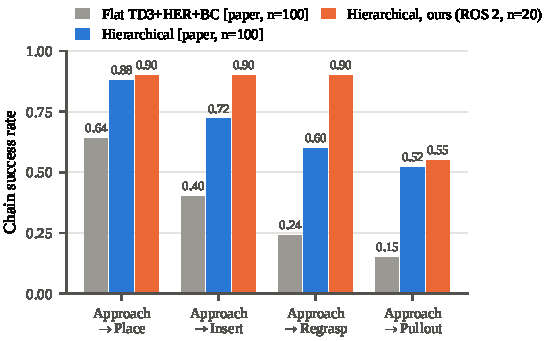
\includegraphics[width=\columnwidth]{hierarchy_chain}
  \caption{Chained success from Approach to each later stage. Grey and blue:
  flat and hierarchical results from~\cite{wu2024surgicai} ($n{=}100$); the flat
  TD3+HER baseline, 0.00 throughout, is omitted. Orange: our replication on
  ROS~2/AMBF~3 ($n{=}20$), with scripted stage sequencing in place of the
  unreleased high-level policy. With $n{=}20$ the 95\% interval on 0.55 is about
  $\pm$0.22.}
  \label{fig:hier}
\end{figure}

The intermediate chains exceed the published values (0.90 against 0.72 and
0.60). The likeliest reason is our stage sequencing: it always retries rather
than letting a learned high-level policy choose, and a retry can recover a
stage that a policy would have abandoned. Table~\ref{tab:scenes} shows why the
policies cannot run on the newer SRC scenes without adaptation. The observations
are absolute poses in the PSM base frame, and the base-to-needle offset changes
by several centimetres between the old and new worlds.

\begin{table}[t]
\caption{What the policies assume, old vs.\ current SRC (static check).}
\label{tab:scenes}
\centering\footnotesize
\setlength{\tabcolsep}{3pt}
\begin{tabular}{@{}p{0.27\columnwidth}p{0.31\columnwidth}p{0.34\columnwidth}@{}}
\toprule
Assumption & Old SRC (policies) & SRC v2.x \\
\midrule
middleware & ROS~1 & ROS~2 \\
needle topic & \texttt{env/Needle} & \texttt{env/phantom/Needle} \\
FK module & \texttt{psmFK} & removed \\
PSM1 base & $(1.0,1.346,1.350)$, 0.1-scaled & $(0.131,0.397,0.878)$\,m \\
needle spawn & hard-coded world pose & differs per phantom \\
\bottomrule
\end{tabular}
\end{table}


%%%%%%%%%%%%%%%%%%%%%%%%%%%%%%%%%%%%%%%%%%%%%%%%%%%%%%%%%%%%%%%%%%%%%%%%%%%%%%%%
\section{PERCEPTION ON THE REAL dVRK}
\label{sec:perception}

\subsection{Simulation-Based Adaptation of Depth Anything for Metric Depth Estimation}
We first evaluated the pretrained Depth Anything V2 model~\cite{yang2024depthv2}
on images from the simulated suturing environment without task-specific
fine-tuning. In this baseline configuration the model produced relative depth
estimates, normalized to a range of approximately 0 to 1, rather than
physically meaningful metric depth. The pretrained model had also never seen
the visual characteristics of the surgical scene: the surgical instruments, the
tissue phantom and the endoscopic imaging conditions. Its depth predictions
therefore had substantial errors and were not accurate enough for downstream
robotic perception and manipulation.

To adapt the model to the surgical domain and make it predict absolute depth
in meters, we fine-tuned it on data generated from the AMBF-based suturing
simulation environment. Collecting equivalent supervised training data directly
from the physical dVRK is difficult because the real endoscopic camera provides
no dense ground-truth depth. The simulator is therefore an effective source of
paired RGB and metric-depth data that preserves the visual and geometric
characteristics of the target surgical scenario.

During data collection, RGB images were acquired from the simulated endoscopic
camera and used as inputs to the depth estimation network. For each RGB frame,
the AMBF simulator also provided a corresponding three-dimensional point cloud.
The 3-D points were transformed into the camera coordinate system and projected
onto the image plane to build a dense per-pixel depth map in meters, which was
used as ground-truth supervision for fine-tuning. Each training sample was thus
an RGB image of the simulated suturing scene paired with its geometrically
derived metric-depth map.

After task-specific fine-tuning, the model estimated depth substantially better
within the suturing environment. Instead of relative depth, the adapted model
predicts depth directly in metric units and reproduces the spatial structure of
the surgical scene more accurately. This simulation-based training strategy is
a practical way to obtain dense depth supervision that is difficult to acquire
on the physical dVRK, and it adapts the pretrained depth estimator to the
geometric and visual characteristics of robot-assisted suturing.
\todo{Jiaming: add the quantitative depth error before and after fine-tuning
(e.g.\ AbsRel, RMSE in mm) and the size of the training set.}

\subsection{FoundationPose Tracking on the Real dVRK System}
\todo{unfinished -- Jiaming: add experimental results and explain the observed
tracking failure.}
FoundationPose~\cite{wen2024foundationpose} was used to estimate the poses of the
PSM and the surgical needle on the physical dVRK. The method requires an RGB
image, an object mask and a depth map as inputs. Because the dVRK endoscope
provides no direct depth measurements, the depth maps were generated with the
fine-tuned Depth Anything model.

The pipeline tracked the surgical needle reliably. Tracking of the PSM was less
stable and had larger pose errors. When tracking the PSM \todo{\ldots}

In simulation, the complete path from RGB through Depth Anything, FoundationPose
and a first-frame physical-plausibility gate to a frozen needle goal passed the
gate on 40/40 captures. A Reach controller driven by these goals succeeded in
29/30 episodes. \todo{Confirm which goal source (GT vs.\ FP) the 29/30 refers
to; these are historical reference runs and were not re-run for this draft.}
Needle yaw in the curriculum is capped at $\pm 30^\circ$ because the pose audit
was reliable at $20^\circ$ but produced near-$180^\circ$ flips at $40^\circ$.
Section~\ref{sec:workspace} shows that this cap, not the policy's trained
workspace, is what limits the task.

\subsection{Hand-Eye Calibration for PSM Localization}
To obtain an independent estimate of the PSM pose in the camera frame, we
performed hand-eye calibration with the dVRK camera registration framework. An
ArUco marker~\cite{garrido2014aruco} was mounted on the PSM shaft approximately
70\,mm from the instrument tip. The camera was positioned so that the marker
stayed near the center of the image, and the PSM was moved through multiple
poses while the marker remained visible. The recorded robot and marker poses
were then used to estimate the transformation between the PSM and camera frames.

This calibration improves the PSM localization accuracy from approximately 5\,cm
to 5--10\,mm. The resulting pose estimate is an additional reference that can
be fused with the FoundationPose estimate, for example with a Kalman filter, to
make PSM tracking more robust. Section~\ref{sec:calib} explains why hand-eye
error of this size is exactly affine in position and can therefore be absorbed
by the grasp calibration.


%%%%%%%%%%%%%%%%%%%%%%%%%%%%%%%%%%%%%%%%%%%%%%%%%%%%%%%%%%%%%%%%%%%%%%%%%%%%%%%%
\section{DEPLOYING THE RELEASED POLICIES}
\label{sec:deploy}

We deploy three checkpoints: the released SurgicAI Approach and Place policies
(TD3+HER+BC) and R6, a locally retrained single-goal Approach policy. Deployment
is inference-only. It uses a CPU-loaded $3{\times}256$ actor and the arm's
\texttt{measured\_cp} in the ECM frame. It does not use AMBF or any training code.

\subsection{The observation--action contract}
The contract is decoded from the checkpoints themselves.

\emph{Observation}: $o=[a,\,d,\,d{-}a]\in\mathbb{R}^{21}$, where $a$ and $d$ are
the achieved and desired poses. Each is written as position in centimetres,
RPY in radians (extrinsic $xyz$, KDL \texttt{GetRPY}), and jaw normalized to
$[0,1]$. Our observation builder reproduces all 502 observations stored in the
R6 checkpoint exactly.

\emph{Action}: $u\in[-1,1]^7$ is integrated as
$c_{t+1}=c_t+u\odot s$. The step $s$ is in \emph{metres} and radians while the
observation is in centimetres, and this asymmetry is part of the contract.

\subsection{Three silent defects}
A deployment can satisfy all of the above and still fail. We replayed each
checkpoint from its own demonstration starts against a kinematic arm model, and
this found three further defects. Together they invalidate every hardware RL
comparison we had made before fixing them.

\emph{1) The roll branch.} A rotation matrix is branch-invariant, but its RPY
triple is not. SciPy returns roll in $[-\pi,\pi]$, whereas SurgicAI's
\texttt{Frame2Vec} maps it into $(-2\pi,0]$. All stored goal rolls in the
released checkpoints lie outside $\pm\pi$, and none lies outside $(-2\pi,0]$.
With the SciPy convention, upstream Approach reproduces 0/25 demonstrations.
The geometric servo was never affected because it uses only relative
rotation. This is why ``the servo works and RL does not'' looked like a
statement about policy quality for so long.

\emph{2) Two action scales.} The environment metadata stores 0.5\,mm\,/\,2$^\circ$,
the scale the \emph{demonstrations} integrate at, and fitting the
demonstrations recovers this value exactly. The training and evaluation scripts,
however, hard-code 1.0\,mm\,/\,3$^\circ$, and all published success rates were
measured at that scale. Replay picks 1.0\,mm\,/\,3$^\circ$ unambiguously
(Fig.~\ref{fig:contract}a). The 1.5\,mm we had been applying came from a
utility module and was never checked against the policy.

\emph{3) Open- vs.\ closed-loop observation.} Inside a subtask, SurgicAI feeds
the network the integrated \emph{command}, never the measured pose. A perfect
arm hides the difference. For a lagging arm, feeding the measured pose drops
Approach from 25/25 to 6/25 at 30\% tracking per cycle
(Fig.~\ref{fig:contract}b). We now compute the observation from an internal
integrator seeded once, and the measured pose is used only by the guards. A
fourth defect appeared while testing this fix. The per-step safety caps were
measured against the measured pose, so they pulled the command back toward a
lagging arm on every cycle. This re-closed the loop from inside the safety
layer. The caps now bound consecutive commands, and a separate guard bounds
tracking error.

\begin{figure*}[t]
  \centering
  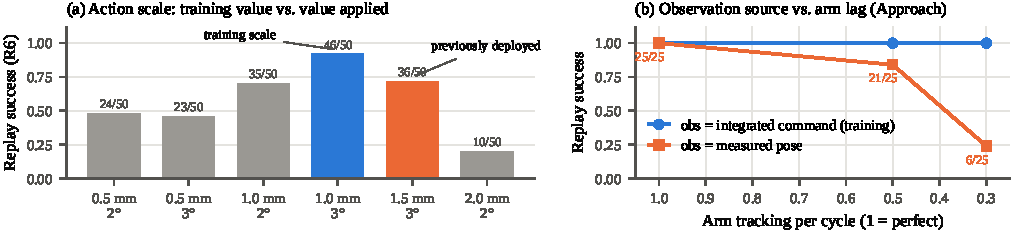
\includegraphics[width=\textwidth]{contract_defects}
  \caption{Two contract defects, measured by replaying policies from their own
  demonstration starts. (a) R6 success as a function of action scale at its own
  tolerance (1\,cm\,/\,10$^\circ$, 200 steps): the training scale gives 46/50,
  and the scale previously deployed gives 36/50. (b) Upstream Approach under a
  first-order lagging arm. Feeding the measured pose instead of the integrated
  command matches the training environment only for a perfect arm.}
  \label{fig:contract}
\end{figure*}

With all three defects fixed, upstream Approach reproduces 45/50 of its
demonstrations through our loop (published $96\pm6\%$), and R6 reproduces 46/50.
We also found that the published rates use a tolerance of
0.5\,cm\,/\,\textbf{30}$^\circ$. At that tolerance Approach reproduces 25/25 and
Place 22/25. At $10^\circ$, the tolerance in the environment metadata, Place
drops to 12/25, so Place is not a precision orientation controller.

\subsection{The workspace question is a staging question}
\label{sec:workspace}
On the real task, the released Approach policy is out of distribution. The
needed start-to-goal rotation is 0--30$^\circ$, while training covered
53--97$^\circ$, and the tool-frame offset has the wrong sign in $y$. Every
unstaged RL run orbited the goal. We first expected this to require retraining
on a wider workspace. However, the demonstrated support of a goal-conditioned
policy is expressed entirely in relative quantities:
\begin{equation}
  \delta = R_s^{\top}(p_g-p_s), \qquad \theta=\angle(R_s,R_g),
\end{equation}
and both are invariant to rigid transforms. For any grasp pose
$(p_g,R_g)$ there is therefore a start pose inside the support, and it can be
solved for directly:
\begin{equation}
  R_s = R_g\,\mathrm{Rel}^{-1},\qquad p_s=p_g-R_s\,\delta^{\star},
\end{equation}
where $\mathrm{Rel}$ and $\delta^{\star}$ are the rotation and offset taken
from the support. We evaluate this on the recorded geometry of our dVRK with
400 needle placements over a $\pm3$\,mm, $\pm30^\circ$ envelope. Without
staging, 0/400 placements are in support. With staging, all 400 are, and the
staging move has a median length of 3.66\,cm and a maximum of 4.14\,cm
(Fig.~\ref{fig:workspace}). For the approach leg, the trained workspace is not
the binding constraint. The binding constraints are perception (the
$\pm30^\circ$ yaw cap), reachability and Place.

\begin{figure}[t]
  \centering
  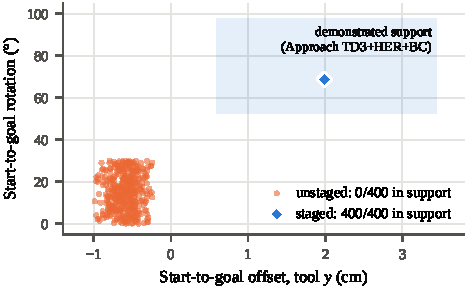
\includegraphics[width=\columnwidth]{workspace_staging}
  \caption{Relative start-to-goal geometry for 400 needle placements on the
  recorded dVRK task, against the demonstrated support of the upstream
  Approach policy. Staging moves every placement to the same point inside the
  support. It is a 3.7\,cm median move, well inside the 8\,cm path-radius
  guard. Computed with \texttt{deploy/tools/workspace\_spec.py}.}
  \label{fig:workspace}
\end{figure}

\subsection{The trained goal is 7\,mm short of the needle}
SurgicAI builds the Approach goal as
$\mathbf{T}_N(\phi)\,\mathrm{Trans}(0,0,7\,\mathrm{mm})\,R_{\mathrm{flip}}$. It is
the grasp point on the arc, backed off 7\,mm along the tool axis with the jaws
pointing at it. In simulation the grasp is then faked by attaching the needle
wherever the jaws are, so no trained motion ever covers the last 7\,mm. On
hardware, closing the jaw at the policy goal would close on empty space. We
therefore add a \emph{descend} phase that covers the standoff at 0.5\,mm per
cycle along the jaw axis with the orientation frozen. It is the slowest motion
in the sequence because it is the only one that can disturb the needle before
the needle is held.


%%%%%%%%%%%%%%%%%%%%%%%%%%%%%%%%%%%%%%%%%%%%%%%%%%%%%%%%%%%%%%%%%%%%%%%%%%%%%%%%
\section{A GUARDED NEEDLE-HANDLING SEQUENCE}
\label{sec:sequence}

\subsection{Phase machine}
Fig.~\ref{fig:phases} shows the sequence. The task is specified by three
\emph{tool} poses in the frame of \texttt{measured\_cp}: the start pose, read
from the arm; the grasp pose; and the suture pose, at which the needle sits
angled at the entry point. Needle-frame targets cannot be used, because after a
blind grasp the needle-in-jaw transform is unknown. The approach leg may use the
RL policy or a staged SE(3) servo (D2). Transport uses the servo. The Place
policy runs in shadow mode only: on the recorded geometry it reports itself out
of distribution as soon as transport begins, which is consistent with its
replay results above.

\begin{figure}[t]
  \centering
  \resizebox{\columnwidth}{!}{% Real-robot phase machine (deploy/surgicai_rl_deploy/sequence.py).
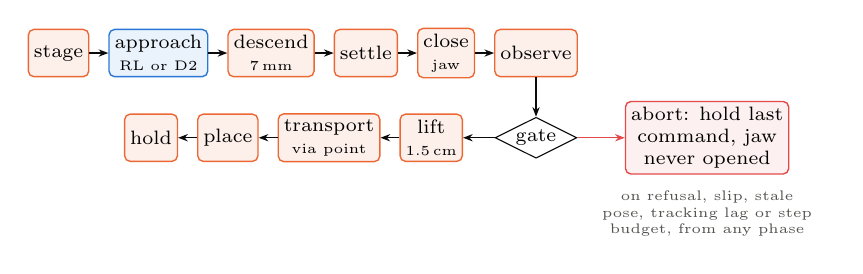
\begin{tikzpicture}[
  font=\scriptsize,
  >={Stealth[length=3.5pt]},
  ph/.style={draw=cOrange, fill=cOrange!10, rounded corners=2pt, minimum height=6mm,
             inner sep=2pt, align=center, line width=0.5pt},
  rl/.style={ph, draw=cBlue, fill=cBlue!10},
  gate/.style={draw=cDark, fill=white, diamond, aspect=2.0, inner sep=0.6pt, align=center},
  stop/.style={draw=cRed, fill=cRed!8, rounded corners=2pt, minimum height=6mm,
               inner sep=2pt, align=center, line width=0.5pt},
  flow/.style={->, draw=cDark, line width=0.5pt},
  note/.style={font=\tiny, text=cMuted, align=center},
  node distance=2.4mm,
]
\node[ph] (stage) {stage};
\node[rl, right=of stage] (appr) {approach\\{\tiny RL or D2}};
\node[ph, right=of appr] (desc) {descend\\{\tiny 7\,mm}};
\node[ph, right=of desc] (settle) {settle};
\node[ph, right=of settle] (close) {close\\{\tiny jaw}};
\node[ph, right=of close] (obs) {observe};
\node[gate, below=5mm of obs] (g) {gate};
\node[ph, left=4mm of g] (lift) {lift\\{\tiny 1.5\,cm}};
\node[ph, left=of lift] (trans) {transport\\{\tiny via point}};
\node[ph, left=of trans] (place) {place};
\node[ph, left=of place] (hold) {hold};
\node[stop, right=6mm of g] (abort) {abort: hold last\\command, jaw\\never opened};

\draw[flow] (stage) -- (appr);
\draw[flow] (appr) -- (desc);
\draw[flow] (desc) -- (settle);
\draw[flow] (settle) -- (close);
\draw[flow] (close) -- (obs);
\draw[flow] (obs) -- (g);
\draw[flow] (g) -- (lift);
\draw[flow] (lift) -- (trans);
\draw[flow] (trans) -- (place);
\draw[flow] (place) -- (hold);
\draw[flow, draw=cRed] (g) -- (abort);
\node[note, below=0.8mm of abort, text width=30mm] {on refusal, slip, stale pose, tracking lag or step budget, from any phase};
\end{tikzpicture}
}
  \caption{The real-robot phase machine. Staging places the arm inside the
  policy's support, and \emph{descend} covers the 7\,mm standoff that training
  never covers. The gate is either a human confirmation (default) or jaw
  evidence. Transport goes through a via point one lift height above the
  suture pose, so the needle cannot pass below the tissue plane. The suture
  pose is corrected for where the jaws actually closed.}
  \label{fig:phases}
\end{figure}

\textbf{No grasp sensor.} The simulator attaches the needle by fiat, and
hardware has no equivalent. Grasp evidence comes from two indirect channels:
the jaw-angle residual relative to an empty-jaw baseline, and jaw effort, which
not every arm publishes. Both are logged with \texttt{grasp\_verified=false}.
The default gate is manual. Jaw units are a further sim-to-real trap: on the
dVRK negative jaw angles mean squeeze, so mapping ``closed'' to 0 applies no
tendon tension at all. The grip is therefore commanded on a separate channel
(default $-15^\circ$).

\textbf{Suture-pose compensation.} A suture pose taught by jogging the arm
while it holds the needle encodes how the needle sat in the jaws at that
moment. Let $W$ be the needle pose, $E$ its required pose and $G$ the grasp.
The tool must reach $S=E\,W^{-1}G$. A pose $S_t$ taught with grasp $G_t$
therefore transfers to an actual grasp $G_a$ as
\begin{equation}
  S_a = S_t\,G_t^{-1}\,G_a ,
\end{equation}
in which neither $E$ nor $W$ appears. Corrections larger than 10\,mm abort,
because a correction that large most likely means the needle moved.

\textbf{Safety envelope.} A fail-closed precheck verifies reachability, the
workspace and operator boxes, step budgets, and tolerances against the lift
distance and the deadband. The operator must state the lift sign, because
$+z$ in the ECM frame is not guaranteed to point away from the tissue. Runtime
guards cap each command at 2.5\,mm and 5$^\circ$, abort on 1.5\,cm of tracking
lag or on a \texttt{measured\_cp} older than 0.25\,s, and never open the jaw on
abort.

\subsection{Hardware bring-up findings}
\textbf{Position deadband.} During the first live staging move, the arm stayed
at 0.25\,cm error for 49 cycles without moving at all. A single hand-published
2\,mm setpoint moved it 1.947\,mm. The loop, however, was publishing about
0.4\,mm per cycle, because a proportional servo shrinks its step near the goal,
and the arm ignored these commands. No existing guard detected this, since the
command never ran more than 0.4\,mm ahead of the arm. We added a minimum command
magnitude that stretches a non-zero command up to the measured deadband, along
the same direction and never past the target. The precheck now rejects any
tolerance finer than the deadband. Fig.~\ref{fig:deadband} reproduces the stall
with a deadband model and shows the fix.

\begin{figure}[t]
  \centering
  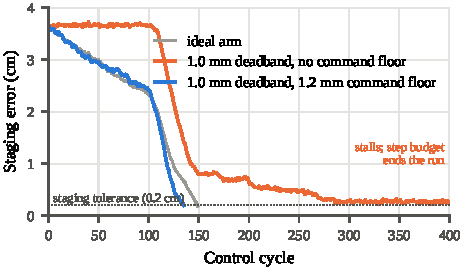
\includegraphics[width=\columnwidth]{deadband}
  \caption{Staging under a 1\,mm position deadband (offline, arm lag 0.5,
  0.2\,mm pose noise). Without a command floor, the servo's shrinking steps are
  absorbed and the move stalls, as on the hardware, until the step budget ends
  the run. A 1.2\,mm floor restores convergence, and the full nine-phase
  sequence completes 0.18\,cm from the suture pose.}
  \label{fig:deadband}
\end{figure}

\textbf{Middleware.} State topics on the dVRK do not all use the same QoS. A
RELIABLE subscriber matched \texttt{measured\_cp} but not
\texttt{jaw/measured\_js}, so the jaw appeared absent even though
\texttt{ros2 topic echo} showed it publishing. All subscriptions now default to
BEST\_EFFORT. The node also refuses to execute when nothing is subscribed to
its command topic, because publishing into the void looks identical to an arm
that does not move.

\textbf{Operator interface.} On the first dry run, the gate prompt printed once
and then scrolled away under a 10\,Hz status line, so the paused arm looked
hung. The prompt now repeats and status output is throttled while waiting.
A keyword-substitution error that reached the node's untested
\texttt{main()} led to static checks. Every keyword and every parsed argument is
now checked against the real signatures using the Python AST. The deployment
package has 588 unit tests, none of which require ROS, a robot or a checkpoint.

\subsection{Offline rehearsal of the full sequence}
Every change is rehearsed against a kinematic arm model with first-order lag,
pose noise, a jaw model and an optional deadband, using the recorded operator
poses. Table~\ref{tab:rehearsal} and Fig.~\ref{fig:sequence} show the full
sequence with the D2 approach controller and the 7\,mm standoff.

\begin{table}[t]
\caption{Offline rehearsal of the full sequence on the recorded task
(D2 approach, 7\,mm standoff, 0.2\,mm noise, seed 1).}
\label{tab:rehearsal}
\centering\footnotesize
\begin{tabular}{@{}lccc@{}}
\toprule
Arm lag per cycle & 0.0 & 0.5 & 0.7 \\
\midrule
Cycles to completion & 166 & 241 & 337 \\
Final error to suture pose (cm) & 0.064 & 0.076 & 0.098 \\
Precheck & pass & pass & pass \\
\bottomrule
\end{tabular}
\end{table}

\begin{figure*}[t]
  \centering
  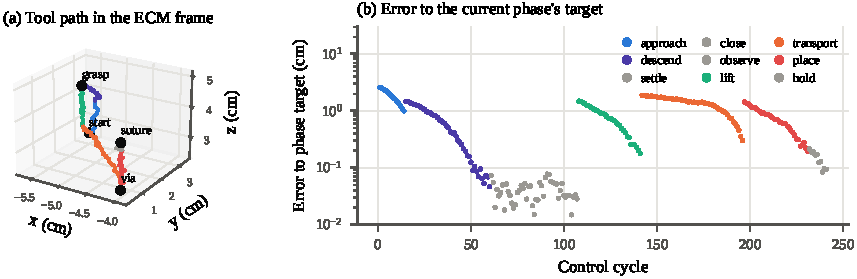
\includegraphics[width=\textwidth]{sequence_rehearsal}
  \caption{One rehearsal of the full sequence (arm lag 0.5). (a) Measured tool
  path in the ECM frame, colored by phase. (b) Error to each phase's own target.
  Every motion phase converges before the next begins, and the jaw phases
  (grey) hold position while the gate is evaluated.}
  \label{fig:sequence}
\end{figure*}


%%%%%%%%%%%%%%%%%%%%%%%%%%%%%%%%%%%%%%%%%%%%%%%%%%%%%%%%%%%%%%%%%%%%%%%%%%%%%%%%
\section{VISION-GUIDED GRASP CALIBRATION}
\label{sec:calib}

\subsection{Two stages}
The coarse stage maps a FoundationPose estimate through the hand-eye transform
to a grasp target $p_{\mathrm{nom}}={}^{E}\mathbf{T}_{C}\,{}^{C}\mathbf{T}_{N}\,
\mathbf{t}_{\mathrm{grasp}}$. The fine stage learns the residual
$r=p_{\mathrm{grasp}}-p_{\mathrm{nom}}$ from grasps taught by hand, following
Xiao~\emph{et~al.}~\cite{xiao2022delta}, with two departures. First, we use
trivariate polynomials of \emph{total} degree~$n$ in the Bernstein basis. The
constant and affine baselines are then the degree-0 and degree-1 rungs of the
same ladder. The model is frame-invariant and needs 1/4/10/20 coefficients
rather than 1/8/27/64 for the tensor-product basis. Second, the penalty is the
exact thin-plate curvature energy, whose null space is the affine functions. As
$\lambda\to\infty$ the fit therefore becomes the affine model, and choosing
$\lambda$ by leave-one-placement-out cross-validation decides whether curvature
has earned its place. The fit is linear and is solved with one QR
factorization. The convex-hull property bounds the correction anywhere in the
calibrated box, and the runtime refuses to extrapolate outside it.

\subsection{Predicted residual structure}
Before collecting any data, we propagate each error source through the dVRK DH
parameters over a 4\,cm grasping box (Fig.~\ref{fig:calib}a). Hand-eye error is
\emph{exactly} affine: $r=(R_{\mathrm{true}}R_{\mathrm{nom}}^{\top}-I)p_{\mathrm{nom}}+b$.
Offsets in the first two PSM joints rotate the whole distal chain about axes
through the base, so they are also affine. Every other geometric term leaves
less than 0.02\,mm after an affine fit, about twenty times below the
repeatability of a taught grasp. A positive result at degree $\geq2$ would
therefore be a statement about FoundationPose's learned bias, not about the
robot. Two choices matter more than the degree. The needle mesh origin is the
centre of the arc, 10.18\,mm from the wire. Using it instead of the SurgicAI
grasp point on the arc raises the cross-validated error from 0.46 to 3.07\,mm at
$\pm30^\circ$ yaw. In addition, the noise floor is correct only when the taught
grasp itself is repeated from a fresh approach. With one grasp per placement the
floor reads 0.31\,mm, while the achieved error is 0.64\,mm. In a power analysis
with a 1\,mm curved bias, 45 placements detected curvature in 6/6 seeds and
produced no false positives at any sample size. We therefore plan 60 placements.

\begin{figure*}[t]
  \centering
  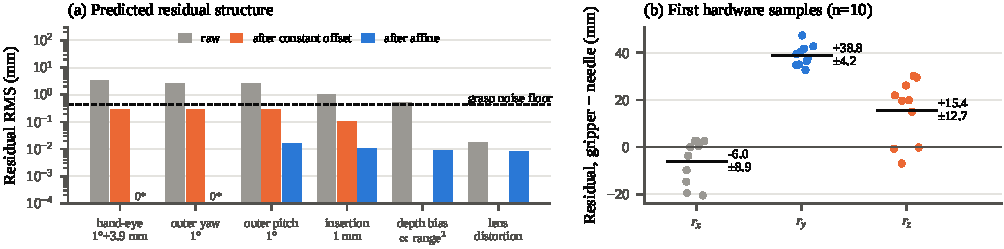
\includegraphics[width=\textwidth]{calibration}
  \caption{(a) Residual RMS over a 4\,cm box predicted from the dVRK kinematics
  for each error source: raw, after removing a constant, and after an affine fit.
  The dashed line is the rehearsed grasp noise floor, and 0* marks terms that are
  exactly affine (${<}10^{-12}$\,mm). (b) Residuals of the first ten hardware
  samples. The near-constant $r_y\approx+39$\,mm (s.d.\ 4.2\,mm, over five days
  and $\sim$150$^\circ$ of wrist variation) points to a frame-definition offset
  rather than to calibration error.}
  \label{fig:calib}
\end{figure*}

\subsection{First hardware samples}
Ten placements have been recorded on our dVRK (Fig.~\ref{fig:calib}b), and none
can yet be used in a fit. \emph{First}, the gripper poses were judged ``ready
to grasp'' by eye, and the jaws were not closed on the needle. The per-axis
correlation between the needle and gripper positions is 0.64, 0.76 and 0.15 for
$x$, $y$ and $z$, the signature of an operator reading depth from a flat
endoscope image. \emph{Second}, the residual contains a constant of about 43\,mm,
mostly in $y$. A constant offset is invisible to a transform-invariant check,
since rigid transforms preserve distances. Our leading hypothesis is a frame
mismatch: \texttt{measured\_cp} is published in an ``ECM'' frame, while the
hand-eye transform maps the camera to the ECM \emph{tip}. Consecutive samples
with the wrist held steady are consistent to within 1.2--1.8\,mm, while samples
taken minutes or days apart are not. The next session will confirm the frame
and collect verified grasps: jaws closed, needle lifted 5--10\,mm, and three
fresh approaches per placement.


%%%%%%%%%%%%%%%%%%%%%%%%%%%%%%%%%%%%%%%%%%%%%%%%%%%%%%%%%%%%%%%%%%%%%%%%%%%%%%%%
\section{DISCUSSION AND LIMITATIONS}

The largest obstacles to transfer were not dynamics or appearance. They were
conventions: an Euler branch, a step size that exists in two versions, whether
the observation closes the loop, a 7\,mm standoff, and the sign of the jaw
angle. Each one looks correct in isolation, and each one fails silently. Our
main methodological recommendation is to measure a deployment contract by
replaying the policy's own demonstrations before running it on a robot, and to
treat any mismatch between replay and the published rate as a bug.

This draft has clear limits. (i) No closed-loop grasp or suture on the real
robot has been completed yet. The hardware results are bring-up findings, dry
runs and calibration samples, and the complete sequence has been validated only
offline. (ii) The hardware RL-versus-servo comparisons made before the contract
fixes are void, and they have not yet been repeated. (iii) The high-level PPO
checkpoint is not available, so the hierarchy results use scripted sequencing,
and $n{=}20$ gives wide intervals. (iv) Place reproduces only 12/25 at a
$10^\circ$ tolerance and does not drive the arm. (v) FoundationPose tracking of
the PSM is not yet reliable (Sec.~\ref{sec:perception}), and the needle-yaw cap
of the pose audit limits the workspace. (vi) Hysteresis is not a function of
position and cannot be represented by any $f(x,y,z)$. Keeping the approach
direction consistent is the only mitigation we apply.


%%%%%%%%%%%%%%%%%%%%%%%%%%%%%%%%%%%%%%%%%%%%%%%%%%%%%%%%%%%%%%%%%%%%%%%%%%%%%%%%
\section{CONCLUSION AND FUTURE WORK}

We replicated the SurgicAI hierarchy on a modern ROS~2 stack and built a
perception front end for the real endoscope. We then made the released policies
executable on a real dVRK PSM through a verified contract, a staging solve and a
guarded phase machine. Next steps, in order: resolve the 43\,mm frame offset and
collect verified grasps; run the empty-gripper rehearsal and then live grasp,
lift and transport with the manual gate; repeat the RL-versus-servo comparison
through the corrected contract; and retrain with start-pose randomization,
which the released Approach demonstrations lack entirely (one distinct start
pose across 50 episodes), and with a Place policy trained to a tight
orientation tolerance.


%%%%%%%%%%%%%%%%%%%%%%%%%%%%%%%%%%%%%%%%%%%%%%%%%%%%%%%%%%%%%%%%%%%%%%%%%%%%%%%%
\section*{APPENDIX}

\textbf{Reproducibility.} The hierarchy replication is on branch
\texttt{jin-hierarchical-repro} of \texttt{xiangruiSun/SurgicAI}
(\texttt{RL/run\_jin\_hierarchical.py}). The deployment, calibration and all
offline tools are in the project repository under \texttt{deploy/}, with the
simulation environments under \texttt{src/SurgicAI/RL/}. The replay numbers
come from \texttt{tools/replay\_demos.py}, the staging analysis from
\texttt{tools/workspace\_spec.py}, the residual structure from
\texttt{tools/residual\_structure.py} and the rehearsals from
\texttt{tools/offline\_grasp\_lift.py}. The script that regenerates every data
figure in this draft is in \texttt{paper/make\_figures.py}.

\textbf{Checkpoint registry.} Upstream Approach TD3+HER+BC
(SHA-256 prefix \texttt{06fc7813f93f}), upstream Place (\texttt{4fc615f07415})
and R6 (\texttt{6286a88c21f0}). All three act at 1.0\,mm\,/\,3$^\circ$.


\section*{ACKNOWLEDGMENT}

We thank the authors of SurgicAI, AMBF and the Surgical Robotics Challenge for
releasing their code and models. \todo{Add lab, hardware and funding
acknowledgments as appropriate.}


\begin{thebibliography}{99}

\bibitem{munawar2019ambf}
A.~Munawar, Y.~Wang, R.~Gondokaryono, and G.~S.~Fischer, ``A real-time dynamic
simulator and an associated front-end representation format for simulating
complex robots and environments,'' in \emph{Proc. IEEE/RSJ IROS}, 2019,
pp.~1875--1882.

\bibitem{munawar2022src}
A.~Munawar, J.~Y.~Wu, G.~S.~Fischer, R.~H.~Taylor, and P.~Kazanzides, ``Open
simulation environment for learning and practice of robot-assisted surgical
suturing,'' \emph{IEEE Robot. Autom. Lett.}, vol.~7, no.~2, pp.~3843--3850, 2022.

\bibitem{wu2024surgicai}
J.~Wu, H.~Zhou, P.~Kazanzides, A.~Munawar, and A.~Liu, ``SurgicAI: A hierarchical
platform for fine-grained surgical policy learning and benchmarking,'' in
\emph{Advances in Neural Information Processing Systems (Datasets and Benchmarks
Track)}, 2024.

\bibitem{yu2024orbit}
Q.~Yu \emph{et~al.}, ``Orbit-Surgical: An open-simulation framework for learning
surgical augmented dexterity,'' in \emph{Proc. IEEE ICRA}, 2024.

\bibitem{review2026rl}
``Applications of reinforcement learning for autonomous surgical robotics: A
systematic review,'' 2026, PMC13511724. \todo{complete citation}

\bibitem{kazanzides2014dvrk}
P.~Kazanzides, Z.~Chen, A.~Deguet, G.~S.~Fischer, R.~H.~Taylor, and
S.~P.~DiMaio, ``An open-source research kit for the da Vinci surgical system,''
in \emph{Proc. IEEE ICRA}, 2014, pp.~6434--6439.

\bibitem{fujimoto2018td3}
S.~Fujimoto, H.~van~Hoof, and D.~Meger, ``Addressing function approximation
error in actor-critic methods,'' in \emph{Proc. ICML}, 2018.

\bibitem{andrychowicz2017her}
M.~Andrychowicz \emph{et~al.}, ``Hindsight experience replay,'' in
\emph{Advances in Neural Information Processing Systems}, 2017.

\bibitem{xie2022randomization}
Z.~Xie \emph{et~al.}, ``Analysis of randomization effects on sim2real transfer in
reinforcement learning for robotic manipulation tasks,'' arXiv:2206.06282, 2022.

\bibitem{chiu2022needle}
Z.-Y.~Chiu, A.~Z.~Liao, F.~Richter, B.~Johnson, and M.~C.~Yip, ``Markerless
suture needle 6D pose tracking with robust uncertainty estimation for autonomous
minimally invasive robotic surgery,'' in \emph{Proc. IEEE/RSJ IROS}, 2022.

\bibitem{wen2024foundationpose}
B.~Wen, W.~Yang, J.~Kautz, and S.~Birchfield, ``FoundationPose: Unified 6D pose
estimation and tracking of novel objects,'' in \emph{Proc. IEEE/CVF CVPR}, 2024.

\bibitem{hwang2020calibrating}
M.~Hwang \emph{et~al.}, ``Efficiently calibrating cable-driven surgical robots
with RGBD fiducial sensing and recurrent neural networks,'' \emph{IEEE Robot.
Autom. Lett.}, vol.~5, no.~4, pp.~5937--5944, 2020.

\bibitem{xiao2022delta}
B.~Xiao, A.~Alamdar, K.~Song, A.~Ebrahimi, P.~Gehlbach, R.~H.~Taylor, and
I.~Iordachita, ``Delta robot kinematic calibration for precise robot-assisted
retinal surgery,'' in \emph{Proc. Int. Symp. Medical Robotics (ISMR)}, 2022.

\bibitem{yang2024depthv2}
L.~Yang, B.~Kang, Z.~Huang, Z.~Zhao, X.~Xu, J.~Feng, and H.~Zhao, ``Depth
Anything V2,'' in \emph{Advances in Neural Information Processing Systems}, 2024.

\bibitem{garrido2014aruco}
S.~Garrido-Jurado, R.~Mu\~noz-Salinas, F.~J.~Madrid-Cuevas, and
M.~J.~Mar\'in-Jim\'enez, ``Automatic generation and detection of highly reliable
fiducial markers under occlusion,'' \emph{Pattern Recognition}, vol.~47, no.~6,
pp.~2280--2292, 2014.

\end{thebibliography}


\end{document}
